\documentclass[tikz]{standalone}
\usetikzlibrary{arrows,positioning}
\newcommand{\tikzsetnextfilename}[1]{}

\definecolor{pGray}{gray}{0.6}

\tikzset{
    circ/.style={circle, draw, inner sep=1pt, minimum width=0.8em, fill=white},
    bg grid/.style={line width=2.5\pgflinewidth, pGray}
}

\begin{document}

\tikzsetnextfilename{6-vertex-model-1}
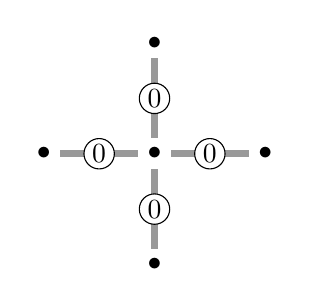
\begin{tikzpicture}[x=2em,y=2em,scale=1.0]
\draw[line width=2.5\pgflinewidth,pGray] (-2,0)--(2,0);
\draw[line width=2.5\pgflinewidth,pGray] (0,-2)--(0,2);
\node[circ,fill=white] at (-1, 0) {$0$};
\node[circ,fill=white] at ( 1, 0) {$0$};
\node[circ,fill=white] at ( 0,-1) {$0$};
\node[circ,fill=white] at ( 0, 1) {$0$};
\node[fill=white] at ( 0, 0) {$\bullet$};
\node[fill=white] at (-2, 0) {$\bullet$};
\node[fill=white] at ( 2, 0) {$\bullet$};
\node[fill=white] at ( 0,-2) {$\bullet$};
\node[fill=white] at ( 0, 2) {$\bullet$};
\end{tikzpicture}

\tikzsetnextfilename{6-vertex-model-2}
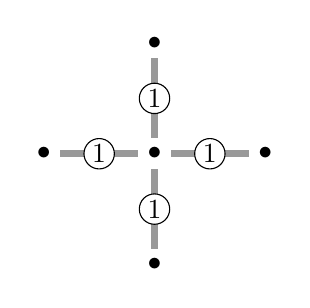
\begin{tikzpicture}[x=2em,y=2em,scale=1.0]
\draw[line width=2.5\pgflinewidth,pGray] (-2,0)--(2,0);
\draw[line width=2.5\pgflinewidth,pGray] (0,-2)--(0,2);
\node[circ,fill=white] at (-1, 0) {$1$};
\node[circ,fill=white] at ( 1, 0) {$1$};
\node[circ,fill=white] at ( 0,-1) {$1$};
\node[circ,fill=white] at ( 0, 1) {$1$};
\node[fill=white] at ( 0, 0) {$\bullet$};
\node[fill=white] at (-2, 0) {$\bullet$};
\node[fill=white] at ( 2, 0) {$\bullet$};
\node[fill=white] at ( 0,-2) {$\bullet$};
\node[fill=white] at ( 0, 2) {$\bullet$};
\end{tikzpicture}

\tikzsetnextfilename{6-vertex-model-3}
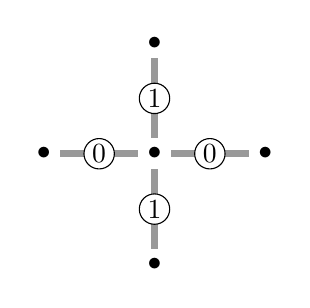
\begin{tikzpicture}[x=2em,y=2em,scale=1.0]
\draw[line width=2.5\pgflinewidth,pGray] (-2,0)--(2,0);
\draw[line width=2.5\pgflinewidth,pGray] (0,-2)--(0,2);
\node[circ,fill=white] at (-1, 0) {$0$};
\node[circ,fill=white] at ( 1, 0) {$0$};
\node[circ,fill=white] at ( 0,-1) {$1$};
\node[circ,fill=white] at ( 0, 1) {$1$};
\node[fill=white] at ( 0, 0) {$\bullet$};
\node[fill=white] at (-2, 0) {$\bullet$};
\node[fill=white] at ( 2, 0) {$\bullet$};
\node[fill=white] at ( 0,-2) {$\bullet$};
\node[fill=white] at ( 0, 2) {$\bullet$};
\end{tikzpicture}

\tikzsetnextfilename{6-vertex-model-4}
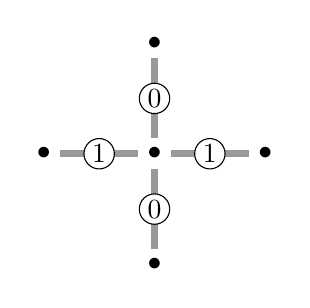
\begin{tikzpicture}[x=2em,y=2em,scale=1.0]
\draw[line width=2.5\pgflinewidth,pGray] (-2,0)--(2,0);
\draw[line width=2.5\pgflinewidth,pGray] (0,-2)--(0,2);
\node[circ,fill=white] at (-1, 0) {$1$};
\node[circ,fill=white] at ( 1, 0) {$1$};
\node[circ,fill=white] at ( 0,-1) {$0$};
\node[circ,fill=white] at ( 0, 1) {$0$};
\node[fill=white] at ( 0, 0) {$\bullet$};
\node[fill=white] at (-2, 0) {$\bullet$};
\node[fill=white] at ( 2, 0) {$\bullet$};
\node[fill=white] at ( 0,-2) {$\bullet$};
\node[fill=white] at ( 0, 2) {$\bullet$};
\end{tikzpicture}

\tikzsetnextfilename{6-vertex-model-5}
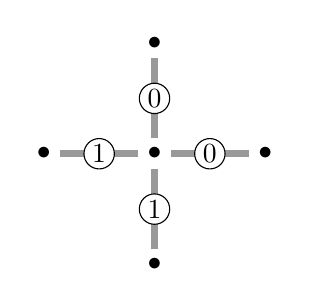
\begin{tikzpicture}[x=2em,y=2em,scale=1.0]
\draw[line width=2.5\pgflinewidth,pGray] (-2,0)--(2,0);
\draw[line width=2.5\pgflinewidth,pGray] (0,-2)--(0,2);
\node[circ,fill=white] at (-1, 0) {$1$};
\node[circ,fill=white] at ( 1, 0) {$0$};
\node[circ,fill=white] at ( 0,-1) {$1$};
\node[circ,fill=white] at ( 0, 1) {$0$};
\node[fill=white] at ( 0, 0) {$\bullet$};
\node[fill=white] at (-2, 0) {$\bullet$};
\node[fill=white] at ( 2, 0) {$\bullet$};
\node[fill=white] at ( 0,-2) {$\bullet$};
\node[fill=white] at ( 0, 2) {$\bullet$};
\end{tikzpicture}

\tikzsetnextfilename{6-vertex-model-6}
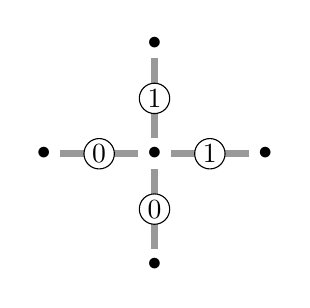
\begin{tikzpicture}[x=2em,y=2em,scale=1.0]
\draw[line width=2.5\pgflinewidth,pGray] (-2,0)--(2,0);
\draw[line width=2.5\pgflinewidth,pGray] (0,-2)--(0,2);
\node[circ,fill=white] at (-1, 0) {$0$};
\node[circ,fill=white] at ( 1, 0) {$1$};
\node[circ,fill=white] at ( 0,-1) {$0$};
\node[circ,fill=white] at ( 0, 1) {$1$};
\node[fill=white] at ( 0, 0) {$\bullet$};
\node[fill=white] at (-2, 0) {$\bullet$};
\node[fill=white] at ( 2, 0) {$\bullet$};
\node[fill=white] at ( 0,-2) {$\bullet$};
\node[fill=white] at ( 0, 2) {$\bullet$};
\end{tikzpicture}

\end{document}

